\subsection{Lancement de l'installation (depuis la console)}
Une fois la machine virtuelle créée, démarrer sur le DVD à jour. Laisser le système se lancer avec les options par défaut. Ensuite, suivre l'assistant d'installation :
\begin{itemize}
    \item Accepter les conditions d'utilisation (figure \ref{fig:03-install-console-01})
    \item Lancer l'installeur (figure \ref{fig:03-install-console-02})
    \item Définir l'interface WAN (figure \ref{fig:03-install-console-03})
    \item La configurer en DHCP (figure \ref{fig:03-install-console-04})
    \item Définir l'interface LAN (figure \ref{fig:03-install-console-05})
    \item Configurer son adresse IP et désactiver le DHCP (figure \ref{fig:03-install-console-06})
    \item Confirmer l'assignation des interfaces (figure \ref{fig:03-install-console-07})
    \item Valider l'emploi de la version communautaire (figure \ref{fig:03-install-console-08})
    \item Choisir le partitionnement par défaut (figure \ref{fig:03-install-console-09})
    \item Ne pas activer de RAID (figure \ref{fig:03-install-console-10})
    \item Confirmer le choix du disque (figure \ref{fig:03-install-console-11})
    \item Redémarrer
\end{itemize}

\begin{figure}[H]
    \centering
    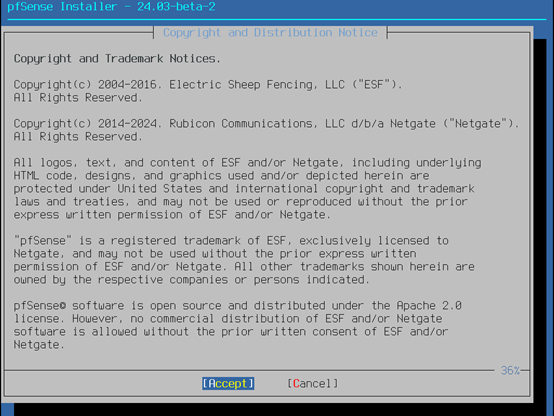
\includegraphics[width=0.88\textwidth]{03-Installation/Images/03-install-console-01.png}
    \caption{Installation - Conditions d'utilisation}
    \label{fig:03-install-console-01}
\end{figure}

\begin{figure}[H]
    \centering
    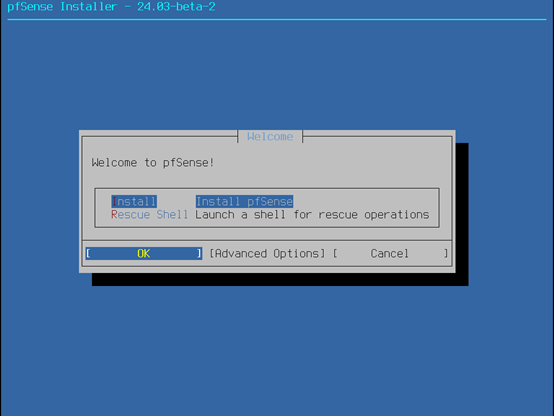
\includegraphics[width=0.88\textwidth]{03-Installation/Images/03-install-console-02.png}
    \caption{Installation - Lancement de l'installation}
    \label{fig:03-install-console-02}
\end{figure}

\begin{figure}[H]
    \centering
    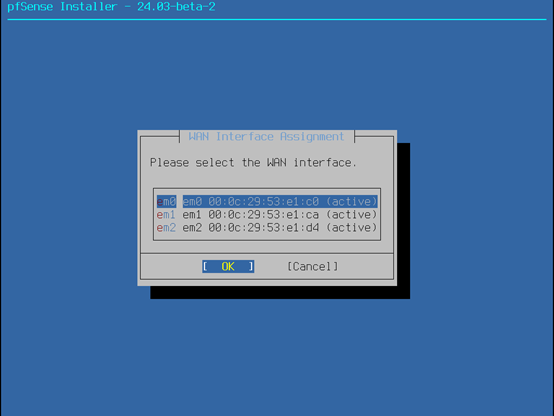
\includegraphics[width=0.88\textwidth]{03-Installation/Images/03-install-console-03.png}
    \caption{Installation - Attribution de l'interface WAN}
    \label{fig:03-install-console-03}
\end{figure}

\begin{figure}[H]
    \centering
    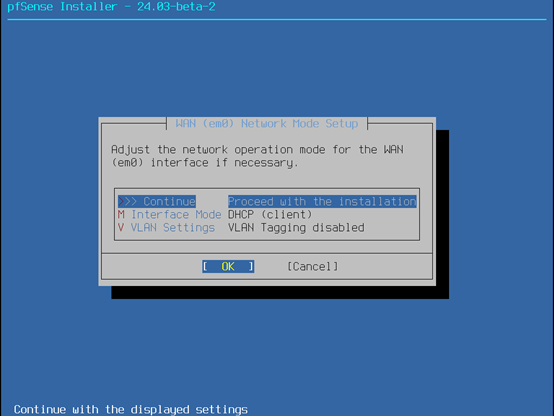
\includegraphics[width=0.88\textwidth]{03-Installation/Images/03-install-console-04.png}
    \caption{Installation - Configuration de l'interface WAN}
    \label{fig:03-install-console-04}
\end{figure}

\begin{figure}[H]
    \centering
    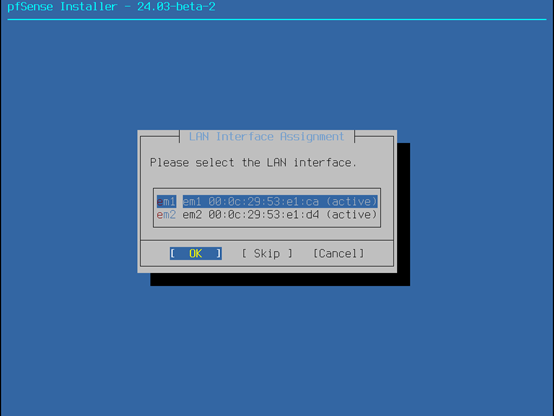
\includegraphics[width=0.88\textwidth]{03-Installation/Images/03-install-console-05.png}
    \caption{Installation - Attribution de l'interface LAN}
    \label{fig:03-install-console-05}
\end{figure}

\begin{figure}[H]
    \centering
    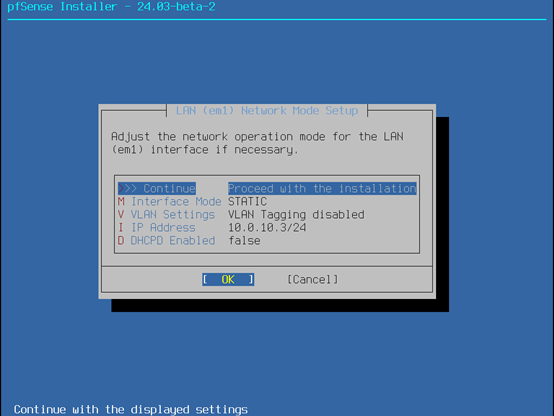
\includegraphics[width=0.88\textwidth]{03-Installation/Images/03-install-console-06.png}
    \caption{Installation - Configuration de l'interface LAN}
    \label{fig:03-install-console-06}
\end{figure}

\begin{figure}[H]
    \centering
    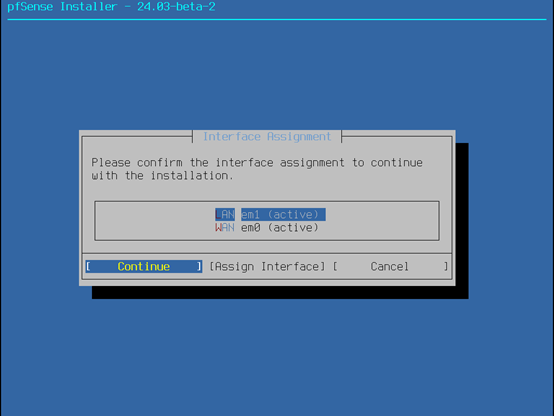
\includegraphics[width=0.88\textwidth]{03-Installation/Images/03-install-console-07.png}
    \caption{Installation - Validation de l'attribution des interfaces}
    \label{fig:03-install-console-07}
\end{figure}

\begin{figure}[H]
    \centering
    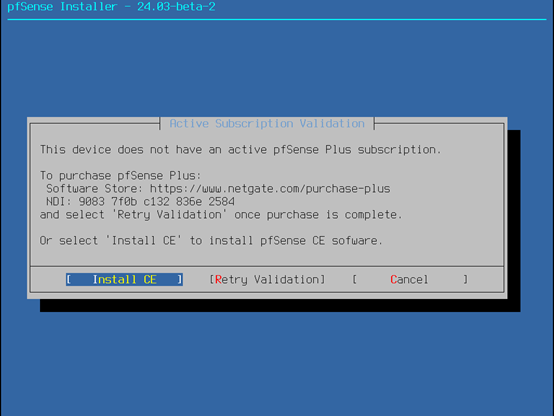
\includegraphics[width=0.88\textwidth]{03-Installation/Images/03-install-console-08.png}
    \caption{Installation - Choix de la souscription au support}
    \label{fig:03-install-console-08}
\end{figure}

\begin{figure}[H]
    \centering
    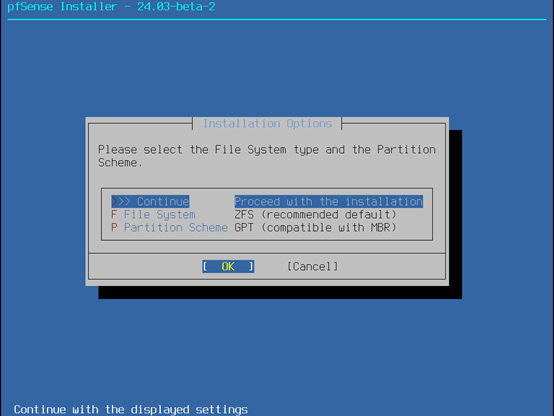
\includegraphics[width=0.88\textwidth]{03-Installation/Images/03-install-console-09.png}
    \caption{Installation - Choix du partitionnement}
    \label{fig:03-install-console-09}
\end{figure}

\begin{figure}[H]
    \centering
    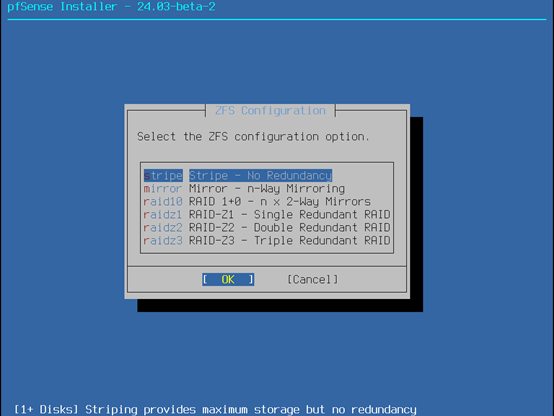
\includegraphics[width=0.88\textwidth]{03-Installation/Images/03-install-console-10.png}
    \caption{Installation - Configuration du RAID}
    \label{fig:03-install-console-10}
\end{figure}

\begin{figure}[H]
    \centering
    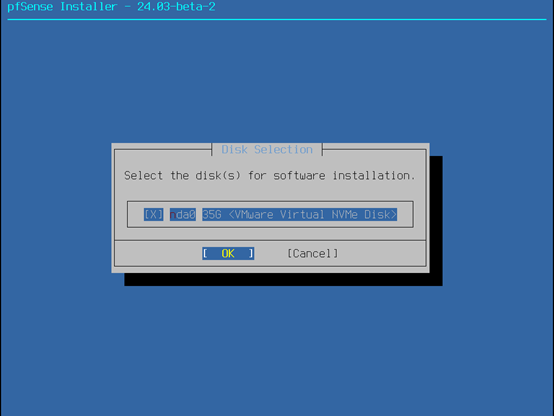
\includegraphics[width=0.88\textwidth]{03-Installation/Images/03-install-console-11.png}
    \caption{Installation - Choix du disque}
    \label{fig:03-install-console-11}
\end{figure}